\section{Introduction}
\label{sec:beam_parameter_chapter_intro}
A gravitational wave creates a differential signal in the arm cavities. The light containing the signal is directed to the \gls{src} (see Section~\ref{sec:detector_chapter_signal_recycling}). This light can be contaminated with non-signal light, i.e.~\emph{junk light}, due to imperfections in the interferometer. This junk light is removed with the \gls{omc} (see Section~\ref{sec:detector_chapter_OMC}), so the light emerging from the \gls{omc} will only contain the signal generated by the differential arm length change. Some of the junk light will come from mode mismatches between the arm cavities and the \gls{src} (see Section~\ref{sec:beam_parameter_chapter_mm_the_arm_to_omc}), and non-optimal mode matching decreases the interferometer's sensitivity (see Section~\ref{sec:beam_parameter_chapter_mm_losses}). The parts of the LIGO detector discussed in this chapter are shown in Figure~\ref{fig:beamparameterchapterligolayout}.
\begin{figure}[h]
	\centering
	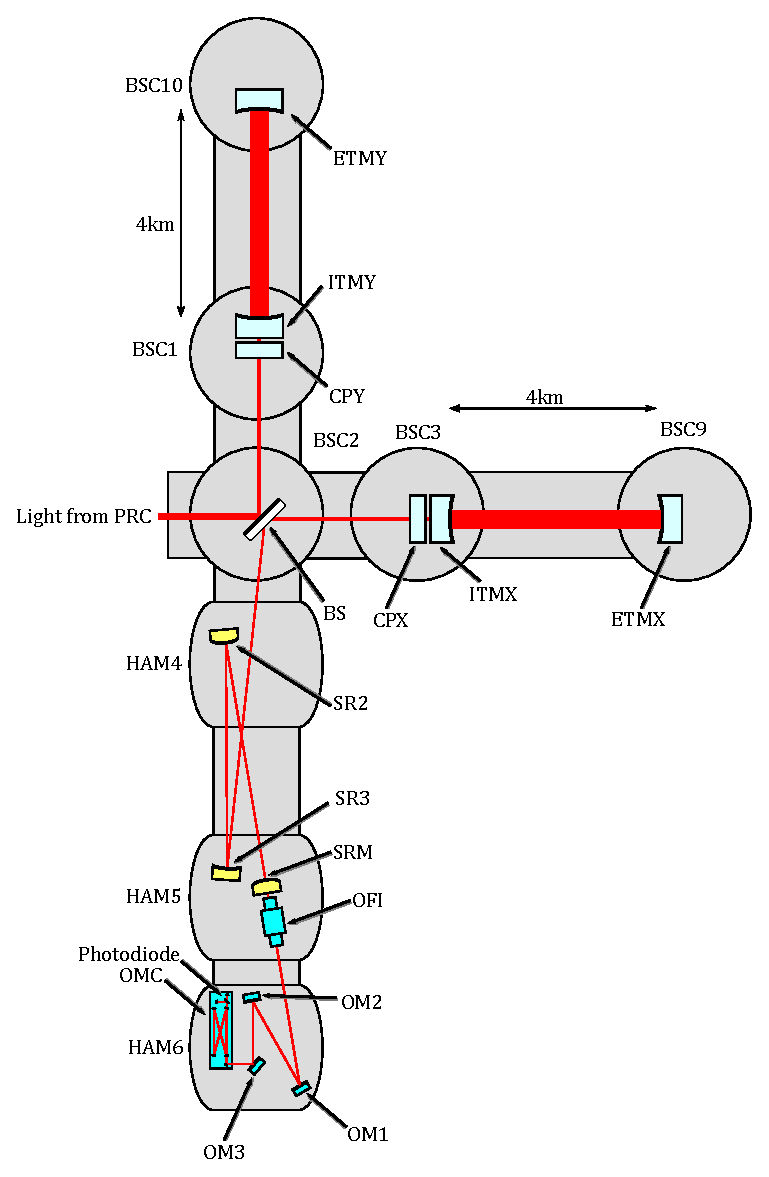
\includegraphics[width=1\linewidth]{Figures/beam_parameter_chapter_ligo_layout}		
	\caption[Sketch showing the parts of the aLIGO detectors discussed Chapter~\ref{chapter:simulation_finesse}.]{Sketch showing the parts of the aLIGO detectors discussed in this chapter. A sketch showing more of the detector is shown in Figure~\ref{fig:ligolayout}. The angles and lengths are exaggerated for clarity. Light from the arm cavities is incident upon the beam splitter (BS). As BS is wedged, the light going towards the \gls{src} comes out an angle. Differential arm length signals encoded onto this light are directed towards SR3, SR2, and then the \gls{srm}. Between the \gls{srm} and the \gls{omc}, there are optics for steering and mode matching (OM1-3). Finally, to strip away junk light, the light enters the \gls{omc}. The light emerging from the \gls{omc} is detected by photodiodes.}%missing	
	\label{fig:beamparameterchapterligolayout}
\end{figure}
\par
Currently, based on the measurements reported on in Section~\ref{sec:beam_parameter_chapter_measurements}, there is significant uncertainty on the arm mode's\footnote{Strictly speaking, there is uncertainty in the beam parameter for both arms' modes at the \gls{srm}. Since the arms are almost identical, the beam parameter is essentially the same for each arm.} beam parameter at the \gls{srm}. The \gls{awc} within HAM6 for LIGO A+ is designed around this uncertainty (see Chapter~\ref{chapter:BHD_for_ligo_2}). 
\par
The effect of errors in the focal length of SR3 and SR2 on the beam parameter and \gls{hom} content of the arm light at the \gls{srm} are explored in this chapter. To do this, a LIGO-like interferometer was simulated using \textsc{Finesse}; this is discussed in Section~\ref{sec:beam_parameter_chapter_finesse_1} and Section~\ref{sec:beam_parameter_chapter_finesse_2}. Using this simulation, the uncertainty in the beam parameter is explored (see Section~\ref{sec:beam_parameter_chapter_beam_parameter_simulation}). 
\par
The difference in the \gls{hom} content of the beam transmitted through the \gls{srm} between an \gls{itm} single-bounce measurement and a measurement which involves the arm cavities is discussed in Section~\ref{sec:beam_parameter_chapter_HOM_simulation}. The effect that the interferometer being in signal recycling and \gls{rse} mode had on the \gls{hom} content of the beam as the focal length of SR3 deviated from its nominal value is also discussed in Section~\ref{sec:beam_parameter_chapter_HOM_simulation}. Section~\ref{sec:beam_parameter_chapter_conclusion} is a summary of the results in this chapter.
%Losses between the arm cavities and the readout photodiodes result in less signal as well as more noise. The decrease in signal is straight forward to understand: if there are less photons to measure, then the signal will be smaller. Since the power is lower, the signal to noise ratio will be larger since shot noise goes as $\sqrt{\rm{Power}}$. As gravitational wave detectors implement squeezing to decrease the quantum noise in the detection quadrature, it is important to preserve the quantum state of the signal field. This means that losses contribute additional noise, as losses pollute the squeezed quantum state with unsqueezed vacuum. \textcolor{red}{This type of loss will be featured earlier in the thesis in the `detector' chapter, so does this need references?}
\subsection{The Mode Matching Between the Arm Cavities, the Signal Recycling Cavity, and the Output Mode Cleaner}
\label{sec:beam_parameter_chapter_mm_the_arm_to_omc}
The \gls{snr} of the gravitational wave signal is directly related to the mode matching between the arm cavities, the \gls{src}, and the \gls{omc}, so it is crucial to have accurate knowledge of the beam parameter at the \gls{srm}. The mode in the arm is well defined since the arm cavities have high finesses. Uncertainties in the \gls{roc} of optics in the \gls{src} telescope (SR2 and SR3, see Figure~\ref{fig:beamparameterchapterligolayout}) results in an uncertainty in the beam parameter of the arm mode at the \gls{srm}, as well as the eigenmode of the \gls{src}. The \gls{src} is a low finesse cavity, so a range of modes that do not match the \gls{src}'s eigenmode can be sustained within it.
\par
Light in higher order modes will be generated if the arms are perfectly matched to the \gls{omc} but not to the \gls{src}. There can be significant mode mismatch between the arms and the \gls{src} and still be lots of signal-light exiting the interferometer because the \gls{src} is a low finesse cavity ($\sim\!15$). If the arms are matched to the \gls{omc} but not to the \gls{src}, then actuators for changing the mode matching between the arm and the \gls{omc} could not be used to increase the differential arm signal sensed by the photodiode after the \gls{omc}. This means the mode matching between the arm and the \gls{omc} can be optimal but the light can still contain \gls{hom}. Additionally, if the beam is astigmatic, then optimal mode matching would not correspond to perfect mode matching.
\subsection{Loss due to Mode Mismatch}
\label{sec:beam_parameter_chapter_mm_losses}
Loss degrades the shot noise limited sensitivity of the interferometer (see Section~\ref{sec:detector_chapter_losses}). It is known that $\sim\!20\%$ of the light is lost between the \gls{as} port and the readout photodiodes, as the shot noise can be compared to the expected shot noise for a given fringe slope, input power and known losses. Approximately half of the loss is accounted for, e.g.~some comes from the \gls{ofi}, some comes from the OM3 pick-off; however, the other half is not fully understood, e.g.~see~\cite{LLO_optical_losses_2018}. The level of squeezing can be used to cross check the loss~\cite{Squeezing_loss_2020}. It is hypothesised that some of the loss which is unaccounted for may come from mode mismatch between the arm cavities and the \gls{omc}.
\par
There are two stages of mode matching ($\rm{Arm}\rightarrow\rm{\gls{src}}$ and $\rm{\gls{src}}\rightarrow\rm{\gls{omc}}$), so the effect of mode mismatch is not simple; this process is known as coherent destructive modal interference~\cite{McCuller2020a}. To model this scenario, it is helpful to consider a Mach-Zehnder interferometer made from theoretical components (modal beam splitters) which split light into the $\rm{HG}_{00}$ and $\rm{HG}_{20}$ and $\rm{HG}_{02}$ modes (i.e~the $\rm{HG}_{20+02}$ mode). \glspl{hom} are discussed in Appendix~\ref{chapter:Light_and_Gaussian_Modes}. The amount of light transferred between the $\rm{HG}_{00}$ and $\rm{HG}_{20+02}$ mode is determined by the magnitude of the mismatch, and the phase difference between the $\rm{HG}_{00}$ and $\rm{HG}_{20+02}$ mode depends on the nature of the mismatch. An error in waist size is in-phase (real), whereas an error in waist location is out-of-phase (imaginary). In general, the mismatch introduces a complex phase. Thus, a sequence of mode mismatches can be modelled in the same way as a Mach-Zehnder interferometer. The difference in phase between the $\rm{HG}_{00}$ and $\rm{HG}_{20+02}$ mode is analogous to a difference in path length in a Mach-Zehnder interferometer. It differs from a typical Mach-Zehnder interferometer as the $\rm{HG}_{00}$ to $\rm{HG}_{20+02}$ splitting ratio is not well balanced. As the loss due to mode mismatches act coherently, the degradation of the squeezed state can be greater for loss due to mode matching than for other types of loss, e.g.~the loss due to photodiodes with a quantum efficiency less than one. If the squeezer is perfectly matched to the \gls{omc}, then the mode mismatch between the squeezer and the interferometer is four times the loss you would expect from treating a mismatch loss as a regular loss. This is explained in detail in~\cite{McCuller2020a,McCuller2020_dcc}.
\subsection{Measurements of the Mode Matching Between the Arm Cavities and the Output Mode Cleaner at the LIGO Livingston Observatory Made Between 2018--2019.}
\label{sec:beam_parameter_chapter_measurements}
The mode matching between the arm cavities and the \gls{omc}, and the input light to the \gls{omc} were studied at the \gls{llo} detector between 2018-2019 by on-site scientists, and these measurements are summarised in Table~\ref{tab:src_chapter_measaurements}. These measurements contradict each other, some suggest that mode matching is near perfect, other suggest it is $\sim\!90\%$. Only one is a direct measurement of the beam profile, which is what we want to know for the design of the \gls{awc} in HAM6 for \gls{bhd} (see Chapter~\ref{chapter:BHD_for_ligo_2}).
\par
Techniques for determining the mode matching between the arms and the \gls{omc} include: actuating on the waist size and waist location of the beam coming from the arm and measuring what effect this has on the mode matching to the \gls{omc}; direct beam profile measurements; the application of different differential arm offsets to determine what portion of light in an \gls{omc} scan corresponds to the arm mode and what portion of the light comes from elsewhere in the interferometer (e.g.~from contrast defect); and measuring a size of a signal known to originate in the arm cavities to find the optimal mode matching configuration for the interferometer. Some of these measurements were performed whilst the arm cavities were locked, and some were made when the interferometer was in \emph{single bounce} mode, i.e.~without the arm cavities being locked.
\begin{table}[h]
	\centering
	\begin{tabular}{|p{25mm} | p{75mm} | c |}
		\hline
		Measurement & Description/Finding & Reference \\
		\hline
		\hline
		Reflectivity of the interferometer. & There is a high amount of mode matching ($>99\%$) between the \gls{prc} and the arm cavities, so single-bounce and locked-arm measurements can be compared. & \cite{interferometer_reflectivity_2019}\\
		\hline
		Mode matching between the arms and the \gls{omc}. & By measuring a signal that originated in the arm and adjusting the mode matching actuators between the arm and the \gls{omc}, the mode matching appears to be within a few percent of perfect. &  \cite{SRM_CO2_chop,CO2_mode_matching_2019} \\
		\hline
		Mode scans of the light incident on the \gls{omc}. & For 10\,W of input power to the interferometer, 11\% of the light incident upon the \gls{omc} was in the $\rm{HG}_{20+02}$ mode. For 40\,W of input power, 4\% of the light was in the $\rm{HG}_{20+02}$ mode. Just after the interferometer lost lock, and thus was in a thermal state similar to how it would be during observation mode, the $\rm{HG}_{20+02}$ content of the light incident on the \gls{omc} was estimated to be 8\%. & \cite{10W_omc_scans_2018,40W_scans_2019,cooling_omc_scan_2018}. \\
		\hline
		Measurement of the beam profile. & A beam profiler was used to measure the size of the beam exiting the \gls{srm}. There was a 15\% mismatch between this beam and the \gls{omc} mode. &\cite{llo_beam_profile_alog_2018,llo_beam_profile_dcc_2018} \\  
		\hline
	\end{tabular}
\caption[Summary of mode matching measurements made at LIGO Livingston by on-site scientist.]{Measurements made at \gls{llo} by on-site scientists of the mode matching between the interferometer and the \gls{omc}.}
\label{tab:src_chapter_measaurements}
\end{table}
%The mode matching between the arm cavities and the \gls{omc}, and the input light to the \gls{omc} were studied at the \gls{llo} detector between 2018-2019, and these measurements are described in the following section. Techniques for determining the mode matching between the arms and the \gls{omc} include: actuating on the waist size and waist location of the beam coming from the arm and measuring what effect this has on the mode matching to the \gls{omc}; direct beam profile measurements; the application of different DARM offsets to determine what portion of light in an \gls{omc} scan corresponds to the arm mode and what portion of the light comes from elsewhere in the interferometer (e.g.~from contrast defect); and use of a beacon signal to distinguish between the signal-carrying arm cavity light and junk light. 
%\par
%Modelling work relies on the mode matching of the \gls{prc} and the arms to be high, and this was estimated from measurements of the interferometer's reflectivity to be $>99\%$~\cite{interferometer_reflectivity_2019}. High amounts of mode matching between the \gls{prc} and the arms allows for single-bounce and full interferometer measurements to be compared. The upper limit on mode matching from the arm to the \gls{omc} is 99\%, and this was obtained from actuation on the beam parameter and the use of a beacon signal (meaning this must be arm cavity light). The entire collection of measurements finds the mode matching to be between 87\% and 99\%. Since this is a large discrepancy, the measurements are briefly discussed below.
%\par
%Mode scans for an input power of 10W find the mismatch to be 11\%~\cite{10W_omc_scans_2018}. The DARM offset was changed to determine what light was coming from the arm mode. An input power of 10W is low, the design is 125W, so the thermal state of the interferometer may be different in this measurement compared to when the interferometer is in observing mode. This method was repeated for 40W of input power\cite{40W_scans_2019}. In this measurement, it was found that there was 4\% mode mismatch.
%\par
%A direct measurement of the beam profile found 15\% mode mismatch between the \gls{omc} waist and the beam transmitted through the SRM while the interferometer was in an ITM single-bounce~\cite{llo_beam_profile_alog_2018,llo_beam_profile_dcc_2018} configuration. This measurement also shows significant astigmatism, with the waist in the x and y directions being separated by $\approx 0.5$\,m. The x direction data is discarded in the analysis as there was trouble orienting the beam profiler. Since there is good mode matching between the input and the arms ($>99\%$), there should not be much difference between this beam and the beam when the interferometer is locked if the thermal lensing in the ITM was similar to how it would be in observation mode. This type of measurement cannot be performed while the arms are locked as they require commissioners to be working near the arm cavities. This analysis is in close agreement with the mode scan measured in~\cite{10W_omc_scans_2018}.
%\par
%Altering the beam parameter using the ITM thermal lens actuator has shown that the mode matching between the arm cavity and the \gls{omc} can be improved by $1\%-2\%$\cite{SRM_CO2_chop}. Actuating on the beam parameter of the arm cavity with the SRM CO2 heater increased the interferometer's optical gain~\cite{SRM_CO2_chop} since the amplitude of the beacon signal increased by 10\%. The ITM and the SRM are separated by sufficient Gouy phase, so actuating on them covers enough beam parameter phase space to determine if the mode matching was optimised. The interferometer was in single-bounce mode, but since the mode matching between the \gls{prc} and arm cavity is high, this is similar to a locked-arm cavity measurement. The interferometer's input power was 25W, so thermal effects may be different between this measurement and when the interferometer is in observation mode. This type of measurement was repeated using 40W of input power\cite{CO2_mode_matching_2019}. Assuming the ITM thermal lens was optimal, the mode matching from the arm to the \gls{omc} was found to be optimal with no SRM heating applied. This suggests that the mode matching is $>99\%$. A beacon signal was used to determine the mode matching between the arm to the \gls{omc}.
%\par
%Modelling of the arm mode finds that a 3.5\% improvement in mode matching between the arm cavity and the \gls{omc} can be made using the ITM thermal lens and the SRM thermal lens~\cite{\gls{omc}_single_bounce_modelling_2018}. This modelling is compared to the measurement made with data from~\cite{llo_beam_profile_dcc_2018}. It was found experimentally that a 4\% improvement in the mode matching between the arm to \gls{omc} could be achieved for a single-bounce measurement with 25W of input power. The interpretation of the measurements in~\cite{\gls{omc}_single_bounce_modelling_2018} contradicts that of~\cite{CO2_mode_matching_2019}, as~\cite{CO2_mode_matching_2019} shows that the mode matching between the arm and the \gls{omc} is optimised.
%\par
%Just after the interferometer had lost lock, a series of mode scans were used to create a model which predicts 92\% mode matching between the beam transmitted through the SRM and the \gls{omc}~\cite{cooling_omc_scan_2018}. The input power was 20W and the lock lasted 1 hour and 41 minutes, so the interferometers thermal state immediately after this lock loss was the same as it would be for a typical time during observing mode when the input power was 20W. The thermal lens in the ITM was measured using the Hartmann wavefront sensors, and this was used to model the interferometer at the time of unlocking. The Hartmann data is noisy, which could cause uncertainty in the mode matching prediction made by the model, although no error on the fit parameters is given in~\cite{cooling_omc_scan_2018}.
%\par
%The mode matching between the squeezer and the optics within HAM6 was studied~\cite{Finesse_model_ham6_2018,sqz_omc_mode_matching}. Measuring the beam profile between the squeezer and the \gls{omc} allows for the layout in HAM6 to be modelled. This means that there is less uncertainty in where the mismatch between the arms and the \gls{omc} originates. The mode matching between the squeezer and the \gls{omc} was measured to be 98\%. The model of HAM6 that was developed from this data differs significantly from the nominal values of the optics in HAM6, a 15\% error in the RoC of OM2 is required to explain the beam profile measurements. This may not be unreasonable, as accurate measurements of focal lengths for mirrors with $f = 2\rm{m}$ are challenging to make.
%\subsubsection{Summary Of Measurements at \gls{llo}}
%Will remove this list?
%\begin{itemize}
%	\item \href{https://alog.ligo-la.caltech.edu/aLOG/index.php?callRep=37742}{\gls{llo} alog 37742}: This is a set of measurements where the DARM offset was changed for an input power of 10W. \gls{omc} scans were used. This finds the mode mismatch to be $\approx13\%$. Date: 17/04/2018.
%	\item \href{https://alog.ligo-la.caltech.edu/aLOG/index.php?callRep=37291}{\gls{llo} alog 37291}: A direct measurement of a beam profile was made for an ITM single-bounce configuration (\href{https://dcc.ligo.org/LIGO-T1800089}{T1800089}) show a large difference between the designed beam and the beam that is transmitted through the SRM. This measurement also shows a fair amount of astigmatism, with the waist in the x and y directions separated by $\approx 0.5$\,m. The x direction data is discarded in the analysis as there was trouble orienting the beam profiler (data available on DCC page). Since there is good mode matching between the input and the arms ($>99\%$), there should be not much difference between this beam and the beam when the interferometer is locked. This type of measurement cannot be performed while the arms are locked as they require commissioner to be working nearby the arm cavities. This analysis agrees with the mode mismatch measured in \href{https://alog.ligo-la.caltech.edu/aLOG/index.php?callRep=37742}{\gls{llo} alog 37742}. Date 09/01/2018.
%	\item \href{https://alog.ligo-la.caltech.edu/aLOG/index.php?callRep=38689}{\gls{llo} alog 38689 (comment)}: This post shows that the beam parameter adjustment that can be made with the thermal lens in the ITM is within $\approx1\%$ of optimal. The interferometer was in single-bounce. It measured the DC transmission through the OMC. Since single-bounce and locked arms are equivalent, this measures arms to OMC mode matching. Date: 18/04/2018.
%	\item \href{https://alog.ligo-la.caltech.edu/aLOG/index.php?callRep=38698}{\gls{llo} alog 38698 (comment)}: This is some modelling work that shows of the order 1\% mismatch between the arms and the OMC. The modelling uses the ITM and and SRM thermal lenses to fit the model beam to the measured beam. It predicts that 3.5\% improvement in arm to OMC modematching can be obtained with the SRM thermal lens, and a 4\% improvement was measured in \href{https://alog.ligo-la.caltech.edu/aLOG/index.php?callRep=38080}{\gls{llo} alog 38080}. It is noted that this modelling does not tie up with \href{https://alog.ligo-la.caltech.edu/aLOG/index.php?callRep=38448}{\gls{llo} alog 38448}, \href{https://alog.ligo-la.caltech.edu/aLOG/index.php?callRep=38240}{38240}, \href{https://alog.ligo-la.caltech.edu/aLOG/index.php?callRep=37893}{37893} and \href{https://alog.ligo-la.caltech.edu/aLOG/index.php?callRep=37742}{37742}. Date: 20/04/2018.
%	\item \href{https://alog.ligo-la.caltech.edu/aLOG/index.php?callRep=41428}{\gls{llo} alog 41428}: This log describes a measurement where the just after the interferometer lost lock, so was in a thermal state similar to when it was locked, the OMC was scanned. This showed that there was $\approx92\%$ mode matching between the input beam to the OMC and the OMC eigenmode when there was 100\,kW of power in the arms. Date: 27/10/2018. 
%	\item \href{https://alog.ligo-la.caltech.edu/aLOG/index.php?callRep=42187}{\gls{llo} alog 42187}: The measured mode matching between the squeezer and OMC is 98\%. This information was used to help model the HAM6 layout, as described in \href{https://dcc.ligo.org/LIGO-T1900159}{T1900159}. There is some uncertainty associated with the HAM6 layout, as this modelling required the radius of curvature (RoC) of OM2 to be significantly different from the nominal value. The beam profile measurements made in \href{https://dcc.ligo.org/LIGO-T1800089}{T1800089} did not require changing the RoC of any mirrors in HAM6. Date: 05/12/2018.
%	\item \href{https://alog.ligo-la.caltech.edu/aLOG/index.php?callRep=43065}{\gls{llo} alog 43065}: This describes a measurement where the SRM CO2 laser heater was used to alter the beam parameter (as its nearly orthogonal to the compensation plate) and found that at 40\,W input power, there was a fraction of a percent effect on the mode matching. This in combination with \href{https://alog.ligo-la.caltech.edu/aLOG/index.php?callRep=38689}{\gls{llo} alog 38689 (comment)} suggest that the mode matching is already close to optimal. \href{https://alog.ligo-la.caltech.edu/aLOG/index.php?callRep=43065}{\gls{llo} alog 43065} also describes how the beacon method of determining mode matching betweeen the arm and the OMC gives $\approx99\%$ mode matching. Date: 07/02/2019.
%	\item \href{https://alog.ligo-la.caltech.edu/aLOG/index.php?callRep=45830}{\gls{llo} alog 45830 and 46029 (comment)}: This shows of OMC scans taken with different DARM offsets. There is 40W of input power to the interferometer. By increasing the amount of light coming from the arms, the amount of junk light that comes from the power recycling cavity due to non-perfect contrast can be measured. This method of measuring mode matching finds $\approx36\%$ higher order modes, $4\%$ of which come from the $\rm{HG}_{20+02}$ mode. Date: 09/05/2019, 17/05/2019.
%\end{itemize}
\section{Modelling Interferometers with Mode Mismatches Using \textsc{Finesse}}
\label{sec:beam_parameter_chapter_finesse_1}
\textsc{Finesse} is software for simulating optical layouts \cite{Freise2004,finesse_manual}. Optical layouts are modelled with components such as mirrors, lenses, and spaces. The way these components are connected is defined by nodes. \textsc{Finesse} performs a nodal analysis to calculate the steady state amplitude of light fields within the optical layout, similar to how a circuit can be analysed. PyKat is a python wrapper for \textsc{Finesse} which provides many quality-of-life improvements such as the ability to programmatically update and re-run simulations~\cite{Pykat}.
\par
The light fields that are calculated in a \textsc{Finesse} simulation can be outputted by using virtual detectors such as a photodiode, \texttt{pd}, or an amplitude detector, \texttt{ad}. These can be configured to detect only certain modes using the \texttt{mask} command. The \texttt{bp} detector is used for outputting the beam parameter, and the \texttt{gouy} command computes the Gouy phase accumulated along a set of spaces. These detectors were used to find the ratio of light in \glspl{hom} to light in the $\rm{HG}_{00}$ mode, the beam parameter of the arm mode that is transmitted through the \gls{srm}, and the Gouy phase accumulated along the \gls{src}.
\par
The beam parameters at nodes in a \textsc{Finesse} simulation are determined by \texttt{cav} and \texttt{gauss} commands. The \texttt{cav} command is used for defining linear and circular cavities. The beam parameters are found by solving for the cavity's eigenmode. Once these nodes have had a beam parameter defined at them, the components connected to them have their beam parameter calculated based on the set of linear equations that define the component. If there are more than one \texttt{cav} commands used in a simulation, the latter \texttt{cav} command overwrites the previous one. The \texttt{gauss} command executes after the \texttt{cav} commands and sets the beam parameter of the laser used in the simulation. 
\par
\textsc{Finesse} can perform simulations using \gls{hg} modes, allowing for the effects of mode mismatches to be modelled if the problem satisfies the paraxial approximation. A coupling between the \gls{hg} modes happens whenever a beam described by $q_1$ enters a segment described by $q_2$. This could happen if the \texttt{gauss} command used on the laser does not correspond to the eigenmode of a cavity defined by the \texttt{cav} command. 
\par
A laser beam can be modelled as a linear combination of \gls{hg} modes. Ideally, an infinite number of these modes would be used in a calculation; however, since it is not feasible to simulate an infinite number of \gls{tem} modes, the maximum number of \gls{tem} modes needs to be defined in a \textsc{Finesse} simulation. This is done using the \texttt{maxtem} command. \textsc{Finesse} will calculate the coupling of the light amongst these modes. If an insufficient number of \gls{tem} modes is used in the simulation, the output will be nonsense because power from the higher order \gls{tem} modes that would be required to accurately model the optical layout will be `aliased' into the ones defined in the simulation. When a cavity becomes unstable, \textsc{Finesse} will not generate physical results since the cavity will not be mathematically describable.
\par
The distance between components, $L$, in a \textsc{Finesse} simulation is defined with a macroscopic distance, $l$, which is modelled with the \texttt{space} command, and a microscopic distance which is modelled with the tuning parameter, $\phi$, belonging to components such as mirrors (\texttt{m}) and beam splitters (\texttt{bs}). The macroscopic distance $l$ is always an integer number of wavelengths, whereas the microscopic tuning, $\phi$, determines the position of a component to sub-wavelength accuracy. \textsc{Finesse} uses the convention that to move a mirror one wavelength, a tuning of $4\pi$\,rad is used. This is so a tuning of $2\pi$ of a mirror in a Fabry-Perot cavity results in the cavity's round trip getting one wavelength longer. It is useful to split the total length, $L = l+\phi$, in this way since the $l$ determines things like Gouy phase whereas $\phi$ determines whether a cavity is on resonance/which mode is resonant. When simulating mode mismatches, the manual states that the command \texttt{phase 2} is required to give physically correct results.
\subsection{Thin and Thick Beam Splitters} 
\textsc{Finesse} is mature software that has been tested against analytic and experimental results. However,
care needs to be taken when using \texttt{Finesse} since incorrect usage can yield erroneous results. Users will get strange results if beam splitters are modelled with just one \texttt{bs} command. In this thesis, such components are called `thin beam splitters'. To illustrate this, two simulations of Michelson interferometers were run, one with a thin beam splitter and the other with a thick beam splitter made up of 3 thin beam splitters and two spaces with a refractive index $>1$. See Figure~\ref{fig:diagramofsim2} for an illustration of a thick beam splitter. The \textsc{Finesse} code for these simulations can be found in Appendix~\ref{sec:finesse_code}.
\par
For a real beam splitter, for energy to be conserved, each reflection from a dielectric coating where the refractive index is lower on the reflecting side than on the transmitting side causes a light field to gain 180\si{\degree} of phase. In a Michelson, there is one path with two of the $\pi$ phase change reflections, while in the other path there is only one such reflection. This means when the arms have equal lengths, destructive interference occurs at the \gls{as} port. The intensity, $I$, at the \gls{as} port of the Michelson as a function of the tuning of one of the arm mirrors, $\Delta \phi$, including the \textsc{Finesse} convention for phase, is
\begin{equation}
	I = I_0\sin^2\left(\Delta \phi \right),
	\label{eq:michelson}
\end{equation}
where $I_0$ is the input power.
\par
The effect of using a thin beam splitter versus a thick beam splitter in a \textsc{Finesse} simulation is shown in Figure~\ref{fig:thinvsthick}. The thin beam splitter causes there to be constructive interference at the \gls{as} port for equal arm lengths, whereas Equation~(\ref{eq:michelson}) shows that it should be destructive interference. Using a thick beam splitter fixes this `bug', as the phase at the beam splitter is accounted for.
\begin{figure}[ht]
	\centering
	
\includegraphics[width=0.95\linewidth]{sim_chapter_thin_vs_thick.eps}
	\caption[\textsc{Finesse} simulation of a Michelson interferometer showing how incorrectly implemented beam splitters can yield erroneous results.]{The simulation of a Michelson interferometer with a thin beam splitter is shown in blue. The same simulation was done with a thick beam splitter and this is shown in orange. The analytic behaviour of a Michelson interferometer (Equation~(\ref{eq:michelson})) is shown by the dashed black line. The tuning of one of the arm mirrors was changed and the power at the \gls{as} port was simulated. Comparing the outputs of the simulation to Equation~(\ref{eq:michelson}) shows that thick beam splitters should be used.}
	\label{fig:thinvsthick}
\end{figure}
\clearpage
\section{Modelling of a Michelson Interferometer with Fabry-Perot Arm Cavities and a Signal Recycling Cavity}
\label{sec:beam_parameter_chapter_finesse_2}
To investigate what effect a mode-mismatch between the \gls{src} and the arm cavities has on the \gls{hom} content of the beam transmitted through the \gls{srm}, a `LIGO-like' interferometer was simulated in \textsc{Finesse}. This interferometer uses two identical, design specification arm cavities. The lengths between the optics in the \gls{src} were obtained from the Zemax model of the \gls{llo} interferometer, and the focal lengths of the optics in the \gls{src} are the measured values for the optics used in the \gls{llo} detector. The reason for using identical arm cavities is to eliminate junk light due to mode mismatch between the arms. The \gls{omc}, \gls{imc}, and \gls{prc} were not included in this simulation as these do not affect the beam in the \gls{src}.  A schematic of the simulation is shown in Figure~\ref{fig:diagramofsim2}. The default focal lengths, transmission coefficients and spacings for this simulation are listed in Table~\ref{tab:nominal simulation}.
\par
To perform \gls{itm} single-bounce measurements, the \glspl{etm} are misaligned. This results in the \gls{itm} having an effective power reflectivity of unity. To replicate this in \textsc{Finesse}, the \texttt{R} for each \gls{itm} was set to 1 minus the loss of the \gls{itm} HR coating. The \gls{etm} and \gls{itm} both have 10\,ppm loss. Because the mode matching between the \gls{prc} and the arms is close to 100\%, this is valid. 
\par
The interferometer was set up to be in DC readout mode. The tuning of the arm mirrors was set so that there was 30\,mW of light emerging from the \gls{as} port when the \glspl{roc} of the optics matched the default values. This is discussed in Section~\ref{sec:etm_tuning}.
\begin{figure}[ht]
	\centering
	
\includegraphics[width=1\linewidth]{sim_chapter_sketch_of_simulation}
	\caption[Schematic of the main simulation in Chapter~\ref{chapter:simulation_finesse}.]{Schematic of the simulation. The dimensions of the schematic are not to scale. The laser light is shown as a red line. Black lines with red beams interacting with them correspond to components such as mirrors and lenses. Important nodes are highlighted with black dots and the associated \textsc{Finesse} commands are shown nearby. Zoom-ins provide more detail for the main beam splitter, ITMy and the \gls{src}. The elongated curled bracket highlights the arm cavity, and the text with it shows how it is implemented in \textsc{Finesse}.}
	\label{fig:diagramofsim2}
\end{figure}
\par
Geometry errors in the \gls{src} cause couplings between the $\rm{HG}_{00}$ mode and \gls{hom}. There are two sorts of errors which cause mode mismatch: \gls{roc} errors and errors in the distance between each of the optics in the \gls{src}. \gls{roc} errors are due to uncertainties in the \gls{roc} of SR3, SR2, the \gls{srm}, and unintended levels of thermal lensing in the \gls{itm} and compensation plate. 
\par
The largest geometry errors in the \gls{src} come from \gls{roc} errors in SR3 and SR2, with both errors affecting the beam in a similar way as there is not much Gouy phase between them. Therefore, to investigate how geometry errors affect the beam transmitted through the \gls{srm}, the \glspl{roc} of SR3 and SR2 were varied.
\par
Certain components have a small impact on the uncertainty in the beam parameter at the \gls{srm}. The thermal lensing in the \gls{itm} is assumed to have a focal length of $+50$\,km, and it would require significant deviation, in the direction of more heating, for this lens to have a large effect. The radius of curvature of \gls{srm} is well enough known that it is not the dominant cause of junk light in the \gls{src}. The spacings between the optics in the \gls{src} are known to a great enough precision, less than $\sim\!1\si{\milli\metre}$, that errors in their locations have a negligible effect.
\par
In an interferometer with arm cavities, a small difference in the lengths between the beam splitter and the \gls{itm} for the X and Y arms, known as a Schnupp asymmetry, is required to make the interferometer controllable. For simplicity, no Schnupp asymmetry was included in this simulation. Since spaces are by default on resonance in \textsc{Finesse}, no Schnupp asymmetry is needed to control the inner Michelson length in the model. The Rayleigh length of the beam at the \gls{itm} is of the order of several hundred metres. This is huge in comparison to the Schnupp asymmetry, which is 8\,cm. The Schnupp asymmetry will therefore have only a small effect on the \gls{hom} content of the beam transmitted through the \gls{srm}, but since the dominant sources of \gls{hom} are \gls{roc} errors in SR3 and SR2, the behaviour of the beam in the \gls{src} can be largely understood without it.
\par
The beam parameter of the input laser was defined so that there was no difference between the single-bounce and the locked arm simulation. To define the beam parameter, the \texttt{gauss} command was used. In this simulation, the mode matching from the laser to the arm cavities should be perfect. The amount used was $99.99999\%$; this was found to be sufficient. See Appendix~\ref{app:appendix_to_SRC_finesse_investigation} for details on how $w_0$ and $z$ were determined for the \texttt{gauss} command used on the laser. The power of the input laser was set to 5\,MW to replicate the amount of power on the main beam splitter.
\par
The \texttt{cav} command was used to set up the arm cavities, although the \texttt{gauss} command used on the laser means the \texttt{cav} command is not required (on the fly testing showed this to be the case). A \texttt{cav} command was not used on the \gls{src} since this forces the beam parameter at the \gls{srm} to be determined by the \gls{src} geometry. An \gls{src} cannot be defined in \textsc{Finesse} using the \texttt{cav} command as one of the end mirrors cannot be properly defined.
\par
The detectors for analysing the mode matching between the nominal arm mode (which matches the laser mode) and the \gls{src} mode were \texttt{pd} and \texttt{ad} with various \texttt{mask} commands applied to them. To detect the total light, no \texttt{mask} was applied. To detect the higher order light, a \texttt{mask [pd] 0 0 0} command was used. This sets the sensitivity of the photodiode to the $\rm{HG}_{00}$ mode to 0. The mode matching is then determined as $1 - \text{HOM}/\text{total light}$. \texttt{maxtem} was set to 6 as this was sufficient to simulate the interferometer accurately while it was stable (see Figure~\ref{fig:maxtemexperiment}). As a cross check, two amplitude detectors were used to detect the $\rm{HG}_{20}$ and $\rm{HG}_{02}$ modes. When plotting the power of the $\rm{HG}_{20+20}$ mode, the square of the \texttt{ad} detector output needs to be taken. The \texttt{bp} detector was used to find the beam parameter. To find the Gouy phase accumulated in the \gls{src} by the $\rm{HG}_{00}$ mode, the \texttt{gouy} command was used.
\par
Both signal recycling and \gls{rse} modes of operation were investigated. The tuning of the \gls{srm} determines whether the interferometer is in \gls{rse} mode or in signal recycling mode. If the interferometer has arm cavities, the \gls{srm} detuning which corresponds to \gls{rse} is 90\si{\degree} while the detuning which gives signal recycling is 0\si{\degree}. For an interferometer without arm cavities, to operate in \gls{rse} mode the \gls{srm} detuning should be set to 0\si{\degree}, while to be in signal recycling mode the detuning of the \gls{srm} should be set to 90\si{\degree}. This is because the reflected light from a cavity has an additional \ang{180} compared to if it was reflecting from a mirror. 
\subsection{Determining Tunings for DC readout}
\label{sec:etm_tuning}
To maintain the same \gls{src} finesse seen by the differential mode for each simulation, the interferometer was set up so that it was on the dark fringe, with 30\,mW of light being transmitted through the \gls{srm}. This was achieved by applying a differential tuning to the \glspl{etm} for simulations with the arm cavities, and a differential tuning to the \gls{itm} for single-bounce simulations. The light transmitted through the \gls{srm} for an interferometer with arm cavities as a function of differential \gls{etm} detuning is shown in Figure~\ref{fig:zoominetmtuning}. For an interferometer without arm cavities, the power transmitted through the \gls{srm} as a function of differential \gls{itm} detuning is shown in Figure~\ref{fig:zoominitmtuning}. The tunings for operating with 30\,mW of light being transmitted through the \gls{srm} are shown in Table~\ref{tab:arm_tuning} and Table~\ref{tab:no_arm_cav_tuning}.
\begin{figure}[ht]
	\centering
	
\includegraphics[width=0.95\linewidth]{sim_chapter_Zoom_in_ETM_tuning.eps}
	\caption[Tunings of the end test masses used to produce a DC offset for the simulations with arm cavities.]{For simulations with the arm cavities, the DC offset is created by tuning the \glspl{etm}. The minimum of the dark fringe is at 0\si{\degree} differential \gls{etm} detuning, as shown by the blue line. A slight offset causes light to be at the \gls{as} port. This result was used to determine tunings for simulating what effect focal length errors in SR3 and SR2 have on the beam transmitted through the \gls{srm}. The orange line and dashed green line show that the beam has a negligible \gls{hom} content.}
	\label{fig:zoominetmtuning}
\end{figure}
\begin{table}[ht]
	\centering
	\begin{tabular}{c |c | c }
		Mirror & \gls{srm} Tuning (\si{\degree}) & Mirror Tuning (\si{\degree})\\
		\hline
		ETMx & 0 & $+2.76\rm{e}-06$ \\
		ETMy & 0 & $-2.76\rm{e}-06$ \\
		ETMx & 90 & $+2.64\rm{e}-05$ \\
		ETMy & 90 & $-2.64\rm{e}-05$ \\ 
	\end{tabular}
	\caption[The tunings used for the arm-cavity simulation to get 30mW of light at the dark port.]{The tunings used for the arm-cavity simulation to get 30mW of light at the dark port.}
	\label{tab:arm_tuning}
\end{table}
\begin{figure}
	\centering
	
\includegraphics[width=0.95\linewidth]{sim_chapter_Zoom_in_ITM_tuning.eps}
	\caption[Tunings of the input test masses used produce a DC offset for the simulations without arm cavities.]{For simulations without arm cavities, i.e.~single bounce simulations, the DC offset is created by tuning the \glspl{itm}. The minimum of the dark fringe is at 0\si{\degree} differential \gls{itm} detuning, as shown by the blue line. A slight offset causes light to be at the \gls{as} port. This result was used to determine tunings for simulating what effect focal length errors in SR3 and SR2 have on the beam transmitted through the \gls{srm}. The orange line and dashed green line show that the beam has a negligible \gls{hom} content.}
	\label{fig:zoominitmtuning}
\end{figure}
\begin{table}[ht]
	\centering
	\begin{tabular}{c |c | c }
		Mirror & \gls{srm} Tuning (\si{\degree}) & Mirror Tuning (\si{\degree})\\
		\hline
		ITMx & 0 & $+0.00709$ \\
		ITMy & 0 & $-0.00709$ \\
		ITMx & 90 & $+0.00074$ \\
		ITMy & 90 & $-0.00074$ \\ 
	\end{tabular}
	\caption[The tunings used for the no-arm-cavity simulation to get 30mW of light at the dark port.]{The tunings used for the no-arm-cavity simulation to get 30mW of light at the dark port.}
	\label{tab:no_arm_cav_tuning}
\end{table}
\clearpage
\section{The Beam Parameter of the Arm Mode at the Signal Recycling Mirror}
\label{sec:beam_parameter_chapter_beam_parameter_simulation}
%\par
%Introduce results...
%\par
%There are two choices of focal length of SR3 which would mode match the arm to the SRM as a Gaussian beam has a maximum radius of curvature at its Rayleigh range. The two mode matching solutions lie either side of this maximum. . Since the gouy phase separation between SR3 and SR2 is quite far from 45\si{\degree}, an error in the focal length of SR3 has a similar effect as an error in the focal length of SR2. This can be visualised with a Collins chart, as shown in Figure~\ref{fig:collinschartsrc}. 
%\begin{figure}
%	\centering
%	\includegraphics[width=0.95\linewidth]{sim_chapter_Collins_chart_src}
%	\caption{Collins chart showing the behaviour of the $1/q$, the inverse of the beam parameter, along the \gls{src}. The blue spot indicates the beam at the transmitted thorugh \gls{itm}. As the beam is far from the waist, it does not evolve much between the \gls{itm} and SR3. Just before reflection from SR3 is shown by the orange spot, and right after is shown by green spot. The red spot is right before reflection from SR2, and purple is from just after reflection from SR2. The brown spot indicates the just before reflection/transmission from the SRM.}
%	\label{fig:collinschartsrc}
%\end{figure}
%\subsection{Beam Parameter at the AR Side of the SRM}
The beam parameter at the \gls{srm} depends on macroscopic quantities such as the distances between mirrors and the \gls{roc} of the optics, rather than microscopic tunings. Therefore, the beam parameter is not affected by the interferometer being in \gls{rse} or signal recycling mode. To estimate the propagation of the mode from the arms to the \gls{srm}, the focal lengths of SR3 and SR2 were varied around three standard deviations of their measured values, and the effect this had on the beam transmitted through the \gls{srm} was determined with a \texttt{bp} detector. %To get beam parametersvalues comparable to \href{https://dcc.ligo.org/LIGO-T1200410}{T1200410}, the fused silica substrate was simulated as a space of 7\,cm was used with a refractive index of 1.45.
\par
The effect of a focal length error in SR3 and SR2 on the width and \gls{roc} of the arm mode at the \gls{srm} is shown in Figure~\ref{fig:beamsizesimulated} and Figure~\ref{fig:beamrocsimulated}. These figures show that the beam parameter depends mainly on the focal length of SR3, although SR2 has a noticeable effect. When the focal lengths of SR3 and SR2 are at their nominal values, the simulated beam has a width of 2.1\,mm, a \gls{roc} of $-3.91\,\rm{m}$, and the Gouy phase accumulated between the \gls{itm} and the \gls{srm} is 18.7\si{\degree}. There is a slight difference between the \gls{roc} found here and the design value of $-3.88\,\rm{m}$; this difference is due to the as-built focal lengths of the optics used in the \gls{src} at \gls{llo} being different from the design values -- small differences such as the $36.00$\,m being the nominal \gls{roc} of SR3 and $(35.97\pm0.01)$\,m being the measured \gls{roc} for SR3 could account for this.
\par
Measurements of the single-bounce beam profile~\cite{llo_beam_profile_dcc_2018} suggests that the beam is much larger at the \gls{srm} than the design value. This would correspond to a positive error in the focal length of SR3, as shown in Figure~\ref{fig:beamsizesimulated}. If the beam were this large, it is unlikely that the \gls{src} would be stable, as shown in Figure~\ref{fig:maxtemexperiment}. The measurement of the beam width found in~\cite{llo_beam_profile_dcc_2018} was obtained under fairly artificial conditions, thus it may not represent the beam parameter of the arm mode when the interferometer is in observing mode. For instance, the thermal state of the interferometer was not similar to how it would be during observing mode. Additionally, ~\cite{llo_beam_profile_dcc_2018} reports that there was difficultly in orienting the beam profiler correctly, and this leads to significant uncertainty in this measurement.
\begin{figure}[ht]
	\centering
	
\includegraphics[width=0.95\linewidth]{sim_chapter_beam_size_sr2_sr3.eps}
	\caption[The Gaussian width of the beam that is transmitted through the signal recycling mirror as a function of the error in the focal length of SR3 and SR2.]{The Gaussian width of the beam that is transmitted through the \gls{srm} as a function of the error ($\pm3\sigma$) in focal length of SR3 and SR2. The Gaussian beam width is strongly dependent on SR3's focal length error, whereas SR2's focal length error is less important. When the beam size is much greater than $\sim\!2.25\,\rm{mm}$, the \gls{src} is unstable (see Figure~\ref{fig:maxtemexperiment}), so this area of the parameter space is unlikely to correspond to the beam at the \gls{srm} at \gls{llo}.}
	\label{fig:beamsizesimulated}
\end{figure}
\begin{figure}[ht]
	\centering
	
\includegraphics[width=0.95\linewidth]{sim_chapter_beam_roc_sr2_sr3.eps}
	\caption[The radius of curvature of the beam that is transmitted through the signal recycling mirror as a function of the error in the focal length of SR3 and SR2.]{The \gls{roc} of the beam that is transmitted through the \gls{srm} as a function of the error ($\pm3\sigma$) in focal length of SR3 and SR2. If the arm cavities and the \gls{src} are well mode matched, then the \gls{roc} of the beam transmitted through the \gls{srm} would be $\frac{5.67\rm{m}}{1.45} = 3.91\rm{m}$.}
	\label{fig:beamrocsimulated}
\end{figure}
\par
Information about the beam parameter of the arm mode can be inferred from the Gouy phase accumulated by the arm mode in the \gls{src}. The Gouy phase as a function of focal length error in SR3 and SR2 is shown in Figure~\ref{fig:gouyphasesr2sr3}. Measurements of Gouy phase of the \gls{src} find it to be 22.81\si{\degree}\cite{SRC_gouy_phase_meas_2019} and 21.3\si{\degree}\cite{SRC_gouy_phase_meas_2018}. These measurements of Gouy phase suggests that the beam at the \gls{srm} is smaller than the design value and has a lower curvature. This Gouy phase also corresponds to a similar amount of $\rm{HG}_{00}$ loss that is measured and simulated (Figure~\ref{fig:TM00_simulated}). 
\par
The Gouy phase accumulated in the \gls{src} is almost entirely dependent on the \gls{roc} of SR3 and SR2; positioning errors of up to 1\,cm of SR3 and SR2 do not affect the Gouy phase significantly. Figure~\ref{fig:gouyphasesr2sr3} shows that it is unlikely that the Gouy phase could be 22.81\si{\degree} in a state where the arm has greater than 90\% mode matching to the \gls{src}, as the \gls{roc} of both SR3 and SR2 would have needed to have been three standard deviations from the measured value. This could be accounted for by a much shorter thermal lens in the \gls{itm} (see Figure~\ref{fig:itmtl}). The measurement of 21.3\si{\degree} of Gouy phase is plausible with the 50\,km thermal lens. The single pass thermal lens was measured to be 38.92\,uD, i.e.~$\approx 25.7$\,km~\cite{cooling_omc_scan_2018}, which corresponds to the design value and the value used in this simulation. 
\par
The focal lengths of SR3 and SR2 can be estimated from the Gouy phase measurement. A normal probability density function was used to model the uncertainties in the focal lengths of SR3 and SR2. This was combined into a 2-D normal distribution. Combinations of SR3 and SR2 that result in 21.3\si{\degree} of Gouy phase were found and the value of the 2-D normal distribution for those combinations was calculated. The maximum value of the resulting probability density function (which is normal) corresponds to the most likely combination of focal lengths for SR3 and SR2, and one standard deviation corresponds to the error. Figure~\ref{fig:sr3sr2likelyvalues} shows that the focal length of SR2 to be $(-3.205\pm0.003)$\,m and the focal length of SR3 to be $(17.971\pm0.002)$\,m.
\begin{figure}[ht]
	\centering
	
\includegraphics[width=0.95\linewidth]{sim_chapter_gouy_phase_sr2_sr3.eps}
	\caption[The Gouy phase of the beam that is transmitted through the signal recycling mirror as a function of the error in the focal length of SR3 and SR2.]{The Gouy phase between the ITMs and the \gls{srm} as a function of the error ($\pm3\sigma$) in SR3 and SR2. When the SR3 focal length error $>6\,\rm{mm}$ and SR2 error is zero, the \gls{src} is unstable (see Figure~\ref{fig:maxtemexperiment}), so this area of the parameter space is unlikely to correspond to the beam at the \gls{srm} at \gls{llo}.}
	\label{fig:gouyphasesr2sr3}
\end{figure}
\begin{figure}[ht]
	\centering
	
\includegraphics[width=0.95\linewidth]{sim_chapter_ITM_TL.eps}
	\caption[The Gouy phase between the input test masses and the signal recycling mirror as a function of the strength of the thermal lensing in the input test masses.]{The Gouy phase between the ITMs and the \gls{srm} as a function of the thermal lens in the ITMs for the default values of SR3 and SR2. The nominal \gls{itm} thermal lens focal lengths are $50\,\rm{km}$, and this corresponds to about 19\si{\degree}. More heating results in a greater thermal lens, however the LIGO detectors compensate for this with the thermal compensation system.}
	\label{fig:itmtl}
\end{figure}
\begin{figure}[ht]
	\centering
	
\includegraphics[width=0.95\linewidth]{sim_chapter_maxtem_experiment.eps}
	\caption[Test used to determine an appropriate number of higher order modes to use in the simulation.]{The percentage of $\rm{HG}_{00}$ light transmitted through the \gls{srm} as a function of SR3's focal length for the Michelson interferometer with Fabry-Perot cavities in its arms was simulated. Each simulation used a different \texttt{maxtem} command. The focal length of SR3 was changed. For focal lengths with a positive error greater than 7.5\,mm, the cavity becomes unstable and \textsc{Finesse} does not produce reliable results. For a stable \gls{src}, the minimum number of \gls{tem} modes needed for sub 1\% accuracy is six.}
	\label{fig:maxtemexperiment}
\end{figure}
\begin{figure}[ht]
	\centering
	
\includegraphics[width=0.95\linewidth]{sim_chapter_SR3_SR2_likely_values.eps}
	\caption[The probability distribution of the focal lengths of SR2 and SR3, and the deduced combination of SR3 and SR2 focal length based on a measurement of the signal recycling cavity’s Gouy phase.]{The measurement error of SR3 and SR2 follows a normal distribution. These were combined to make a 2-D normal distribution. Dark blue corresponds to the least likely combinations of SR3 and SR2, and bright yellow corresponds to the most likely. The measured Gouy phase was 21.3\si{\degree}\cite{SRC_gouy_phase_meas_2018}; this is indicated by the white dashed line. The white circle marks the most likely combination of SR3 and SR2 which gives 21.3\si{\degree} of Gouy phase, and the white crosses show one standard deviation from this. The white circle and crosses indicate that the focal length of SR2 is $(-3.205\pm0.003)$\,m and the focal length of SR3 is $(17.971\pm0.002)$\,m.}
	\label{fig:sr3sr2likelyvalues}
\end{figure}
\par
The beam parameter at the \gls{srm} is determined by the focal length of SR3 and SR2, and the focal lengths of SR3 and SR2 have a probability density associated with them (see Figure~\ref{fig:sr3sr2likelyvalues}). Thus, each beam width and \gls{roc} pair that was computed in this simulation also had a probability density associated with it. Based on the measurement of Gouy phase, the beam is likely to have a width of 1.84\,mm and a defocus of -2.80\,Dioptre. This is shown in Figure~\ref{fig:sim_chapter_beam_parameter_at_SRM}. This is a slight simplification as the beam parameter cannot be such that the Gouy phase of the cavity becomes too small (less than $\sim\!17.5\si{\degree}$). The cavity will be unstable if the Gouy phase is too small, so beam widths of more than 2.25\,mm are unlikely. The shape of the distribution of the arm mode beam parameter at the \gls{srm} is driven mostly by the focal length error of SR3.
\begin{figure}[ht]
	\centering
	
\includegraphics[width=0.95\linewidth]{sim_chapter_beam_parameter_at_SRM.eps}
	\caption[Distribution of beam parameters at the signal recycling mirrors.]{The beam parameter at the \gls{srm} was calculated for combinations of SR2 and SR3 focal lengths. The associated probability density for these combinations can be calculated (see Figure~\ref{fig:sr3sr2likelyvalues}), so the probability of the beam parameter having a certain width and defocus can be calculated. The probability density for each pair of beam width and defocus is indicated with the colour bar. The mode corresponding to the measurement of 21.3\si{\degree} of Gouy phase\cite{SRC_gouy_phase_meas_2018} is indicated with a green cross (1.84\,mm, -2.80 Dioptre). This is a simplified approach since the beam parameter cannot be such that the \gls{src} is unstable, so certain combinations of beam width and beam defocus are not possible. Beam parameters with a width greater than $\sim\!2.25\,\rm{mm}$ result in an unstable \gls{src}, therefore these beams are unlikely to be present at the \gls{srm} at \gls{llo}.}
	\label{fig:sim_chapter_beam_parameter_at_SRM}
\end{figure}
\clearpage
\section{Power Transmitted Through the Signal Recycling Mirror for a Mode Mismatch Between the Arm Cavity and the Signal Recycling Cavity}
\label{sec:beam_parameter_chapter_HOM_simulation}
The \gls{hom} content of the beam as a function of the error in focal length in SR3 was investigated. As the arm cavities become more mismatched to the \gls{src}, less $\rm{HG}_{00}$ mode is transmitted through the \gls{srm}. The mode mismatch can be seen in Figure~\ref{fig:TM00_simulated}. As the focal length of SR3 becomes further from its nominal value, the radius of curvature of the beam at the \gls{srm} stops matching the radius of curvature of the \gls{srm}. Since the \gls{src} is a low finesse cavity, a significant mismatch can be tolerated before there is a large drop in the $\rm{HG}_{00}$ power transmitted. This is shown in Figure~\ref{fig:TM00_simulated}. In Figure~\ref{fig:TM00_simulated} and Figure~\ref{fig:allpowerout}, it is shown that the nominal focal length of SR3, $17.985\,\rm{m}$, is longer than optimal. When the \gls{src} is on resonance, the peak in transmission is $-3\,\rm{mm}$ from the nominal focal length of SR3. This is shown by the blue and green lines in Figure~\ref{fig:allpowerout}. 
\par
The power of the $\rm{HG}_{00}$ light transmitted through the \gls{srm} as a function of focal length error is shown in Figure~\ref{fig:allpowerout}. In signal recycling mode, shown as blue and green in Figure~\ref{fig:allpowerout}, the transmitted power has a peak shape. This is because an error in the focal length of SR3 moves the cavity off resonance. In \gls{rse} mode, shown as red and orange in Figure~\ref{fig:allpowerout}, a change in focal length of SR3 does not have much effect on the amount of $\rm{HG}_{00}$ transmitted by the \gls{srm} since an anti-resonance is a much broader feature than a resonance.
\par
In a single-bounce measurement, the beam incident onto the \gls{itm} from outside the cavity is reflected straight back. This is equivalent to the reflectivity of the \gls{itm} being $R = 1$. When the light is resonant in the arm cavity, the \gls{itm} acts as a highly reflective mirror which applies a frequency-dependent phase shift to the light. Thus, there is no difference between a single-bounce measurement and a measurement with arm cavities at frequencies within the linewidth of the cavity. This is shown in Figure~\ref{fig:TM00_simulated}. \gls{hom} beams generated by errors in the \gls{src} are not suppressed by the arm cavities as they are reflected by the \gls{itm}.
\par
The ratio of the light in the $\rm{HG}_{00}$ mode versus the total light depends on the detuning of the \gls{srm}, rather than the presence of cavities in the arm. This is shown in Figure~\ref{fig:TM00_simulated}. When the light enters the arm cavities, it is reflected with an extra $\pi$\,rad phase; however, the \glspl{hom} do not enter the cavity, so they do not acquire this phase. Since the \glspl{hom} only interact with the \gls{src}, the ratio of \gls{hom} to $\rm{HG}_{00}$ depends on the detuning of the \gls{srm} rather than whether the interferometer is in signal recycling or \gls{rse} mode. The amount of higher order mode generated in the \gls{src} is proportional to the $\rm{HG}_{00}$ power in the \gls{src}, so the percentage of \gls{hom} beam is dependent only on the tuning of the \gls{srm} and the focal length error of SR3. 
\par
As the \gls{src} gets closer to being unstable, more \gls{tem} modes are required to simulate the behaviour of the cavity. The effect of using more \gls{tem} modes in the simulation is shown in Figure~\ref{fig:maxtemexperiment}. For positive errors above 6\,mm in the focal length of SR3, the cavity becomes unstable. It was found empirically that six \gls{tem} modes is sufficient to simulate the interferometer while it is stable. The hatched regions of Figure~\ref{fig:TM00_simulated} and Figure~\ref{fig:allpowerout} show where the simulation is not accurate.
\begin{figure}[ht]
	\centering
	
\includegraphics[width=0.95\linewidth]{sim_chapter_TM00_simulated.eps}
	\caption[The percentage of light that is in higher order modes as a function of the focal length of SR3.]{The percentage of light which is in the $\rm{HG}_{00}$ mode as the focal length of SR3 changes compared to the total light power does not depend on whether there are arm cavities. It is determined by the detuning of the \gls{srm}. The blue dashed line shows the behaviour of the beam with arm cavities present and with the \gls{src} in signal recycling mode (\gls{srm} $\phi = 0\si{\degree}$). The red line shows how the beam changes with focal length error for a single-bounce measurement and with the \gls{src} in \gls{rse} mode (\gls{srm} $\phi = 90\si{\degree}$). The orange dashed line corresponds to the interferometer having arm cavities and being in \gls{rse} mode (\gls{srm} $\phi = 90\si{\degree}$). The green line shows the behaviour of the beam when the interferometer is configured for a single-bounce measurement and is in signal recycling mode. The hatched region indicates where the \gls{src} becomes unstable (see Figure~\ref{fig:maxtemexperiment}), so the behaviour of the interferometer cannot be accurately simulated for these focal lengths.}
	\label{fig:TM00_simulated}
\end{figure}
\begin{figure}[ht]
	\centering
	
\includegraphics[width=0.95\linewidth]{sim_chapter_All_power_simulated.pdf}
	\caption[Simulated power of the beam's fundamental mode and the power in its higher order mode as the mode mismatch is changed.]{The total power transmitted through the \gls{srm} for each simulation is shown by the thick pale lines. The thin solid lines correspond to the power in the $\rm{HG}_{00}$ mode, and the thin dashed lines correspond to the power in the higher order modes. Blue lines show the behaviour when the interferometer has arm cavities and is in signal recycling mode, and the orange lines shows when it is in \gls{rse} mode. Green lines show how the power changes when the interferometer is configured for a single-bounce measurement and is in signal recycling mode, and the red line shows when its in \gls{rse} mode. The hatched region indicates where the \gls{src} becomes unstable, and so the behaviour of the interferometer cannot be accurately simulated for these focal lengths.}
	\label{fig:allpowerout}
\end{figure}
\clearpage
\subsection{Change of Finesse of the Signal Recycling Cavity}
As the transmission of the \gls{srm} decreases, the finesse of the cavity increases. A \textsc{Finesse} simulation was run to see the effect of increasing the power transmission of the \gls{srm}. The $\rm{HG}_{00}$ mode power decreases with lower \gls{srm} transmission slower than the power transmitted in the $\rm{HG}_{20+02}$ mode. This is shown in Figure~\ref{fig:srmthgratio}.
\begin{figure}[ht]
	\centering
	
\includegraphics[width=0.95\linewidth]{sim_chapter_SRM_T_HG_ratio.eps}
	\caption[Ratio of power in the fundamental mode and the power in higher order modes as the signal recycling mirrors reflectivity changes.]{Ratio of $\rm{HG}_{20+02}$ to $\rm{HG}_{00}$ as the transmission of the \gls{srm} is increased for a mode mismatch between the arm cavities and the \gls{src}. The interferometer is in \gls{rse} mode. A mode mismatch was introduced by setting the focal length of SR3 to be 12\,mm shorter than the default amount.}
	\label{fig:srmthgratio}
\end{figure}
\section{Conclusion}
\label{sec:beam_parameter_chapter_conclusion}
The mode mismatch between the arm cavities and the \gls{src} results in a loss mechanism whereby light is scattered from the $\rm{HG}_{00}$ mode into higher order modes. Loss in interferometers usually reduces the \gls{snr} by $\sqrt{\rm{Power}}$, however since there are multiple points between the squeezer and the \gls{omc} where mode mismatches can happen, coherent destructive modal interference will cause the losses to have up to four times the effect they would have if it were a normal type of loss. There exists a collection of measurements which shows the arms are matched between $90$\% and $100$\% to the \gls{omc}. 
\par
\textsc{Finesse} simulations were used to model mode mismatches between the arm and the \gls{src} caused by \gls{roc} errors in SR3 and SR2. The simulation used as-built parameters for the \gls{src} at the \gls{llo} site and design specification arm cavities. This allowed us to study the effect of non-ideal mode matching in a close to real life situation. The interferometer was modelled in signal recycling mode and \gls{rse} mode for locked-arm-cavities and single-bounce configurations.
\par
It was found that the dependence of the ratio of $\rm{HG}_{00}$ light to the total light depends mainly on the focal length of SR3 and is not affected by the presence of arm cavities. This is because the arm cavities are well matched to the input laser. When the arm cavities are on resonance, the ITMs act as highly reflective mirrors with frequency dependent behaviour. This means if the interferometer's thermal state remains the same, there is no difference in \gls{hom} content of the beam transmitted through the \gls{srm} between a single-bounce measurement and an arm-cavity measurement. 
\par
The ratio of \gls{hom} to $\rm{HG}_{00}$ for the beam emerging from the \gls{srm} depends on the detuning of the \gls{srm}, although it does not depend on whether the interferometer is in signal recycling mode or \gls{rse} mode. As \glspl{hom} do not enter the arm cavities, they cannot distinguish between the signal recycling and \gls{rse} modes of operation. When the \gls{src} is on resonance, it is much more sensitive to an error in SR3's focal length than when the \gls{src} is anti-resonant. The light is less sensitive to an error in the focal length of SR2. 
\par
The uncertainty in the beam parameter of the arm mode at the \gls{srm} and the eigenmode of the \gls{src} is driven by the uncertainty in SR3. This is shown in Figure~\ref{fig:beamsizesimulated} and Figure~\ref{fig:beamrocsimulated}. The single pass Gouy phase of the \gls{src} for different combinations of SR3 and SR2 was simulated; this is shown in Figure~\ref{fig:gouyphasesr2sr3}. The Gouy phase acquired in a single pass of the \gls{src} was measured to be $(21.3\pm0.3)\si{\degree}$, so it can be inferred that the focal length of SR2 is $(-3.205\pm0.003)$\,m and the focal length of SR3 is $(17.971\pm0.002)$\,m. This is shown in Figure~\ref{fig:sr3sr2likelyvalues}. These values of focal length would result in the arm mode having a width of $1.8$\,mm and a defocus of $-0.28,\rm{m}^{-1}$ immediately after it is transmitted through the \gls{srm}, and there would be a few percent \gls{hom} in \gls{omc} scans (see Figure~\ref{fig:sim_chapter_beam_parameter_at_SRM}).
\par
Future work could involve using a heater to change the focal length of SR3 and measuring the effect this has on the Gouy phase accumulated in the \gls{src}. This measurement could be used to validate the model of the geometric properties of the \gls{src}. As the lengths between all the optics is well known, and the focal length of the ITMs is well known, the squeezer beam could be used to gain information about the \glspl{roc} of SR3 and SR2. This would be done by setting up a single-bounce measurement. Having greater confidence in the beam parameter of the arm mode at the \gls{srm} would be of great benefit for the design of future upgrades, such as balanced homodyne detection (see Chapter~\ref{chapter:BHD_for_ligo_1} and Chapter~\ref{chapter:BHD_for_ligo_2}), to the LIGO detectors.
